\chapter{Week 6: 27\textsuperscript{th} Oct  - 2\textsuperscript{nd} Nov }

 \tocless\section{Objectives}



\begin{itemize*}
	\item Create the state space equations for the roll and pitch.
	\item Make the Simulink model for the Kalman Filter.
\end{itemize*}

 \tocless\section{Derivation of state space equations for Kalman filter}
The following kalman equation was taken from the \cite{Artofcontrol} and can be seen on page 483 and the derivation of the equation can be seen on page 791 of the same book
\begin{equation}
\hat{\bf x}_{k+1|k+1} = \Phi\hat{\bf x}_{k|k} + {\bf \varDelta u}_{k} + {\bf K}[{\bf z}_{k+1} - {\bf C}(\Phi \hat{\bf x}_{k|k} + {\bf\varDelta u }_k) ] \label{eq : kalman gain from art of control long}
\end{equation}

\ref{eq: kalman equation from art of control } is the same \ref{eq : kalman gain from art of control long} but the matrix/variables are grouped together for ease of computation.
\begin{equation}
	\hat{\bf x}_{k+1|k+1} = [{\bf I -KC}][\Phi \hat{\bf x}_{k|k} +\varDelta{\bf u}_k] + {\bf Kz}_{k+1} \label{eq: kalman equation from art of control }
\end{equation}

\ref{eq: kalman equation from art of control } can be written as follows.
\begin{equation}
	\hat{\bf x}_{k+1|k+1} = { F}\hat{\bf x}_{k|k} + { H}{\bf u}_k + {\bf Kz}_{k+1} \label{Eq: Kalman Equation Representation used in our report}
\end{equation}
Where in \ref{Eq: Kalman Equation Representation used in our report} ${ F} =  [{\bf I -KC}]\Phi$; $H =  [{\bf I -KC}]\varDelta $. Thus each matrix is made up of a mix of prediction and current value with the exception of the Kalman gain $\bf K$.

 
\begin{equation}
	\begin{bmatrix}																
		\hat{x}_1		         			\\
		\hat{ x}_2		
		\end{bmatrix}_{k+1}
		=
	\begin{bmatrix}
		F_{11}	& F_{12 } \\
		F_{21}	& F_{22}
		\end{bmatrix}
			\begin{bmatrix}											
			\hat{\bf x}_1		         			\\
			\hat{\bf x}_2		
			\end{bmatrix}_{k}	
			+
	\begin{bmatrix}
	H_1 \\
	H_2
	\end{bmatrix}
	{\bf u}_k
	+
	\begin{bmatrix}
	K_{11}	& K_{12 } \\
	K_{21}	& K_{22}
	\end{bmatrix}
	\begin{bmatrix}											
	{ z}_1		         			\\
	{z}_2		
	\end{bmatrix}_{k+1}	
\end{equation}

{\bf Where:} ${\bf x_1}$ is angular velocity ${\bf \alpha}$ and ${\bf x_2}$ is angular acceleration $\dot{\bf \alpha}$  

\newpage
 \tocless\section{Simulink model of Kalman filter}
\begin{figure}[h]
	\centering
	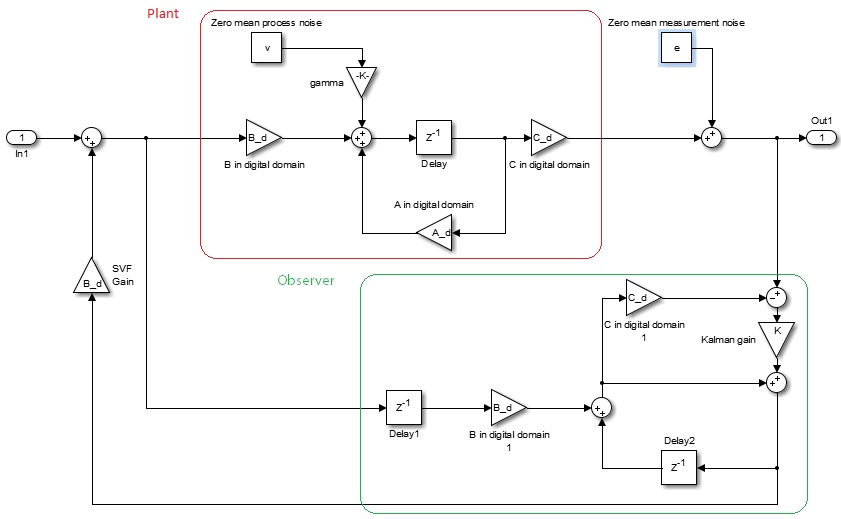
\includegraphics[scale = 0.5]{\DocRoot/images/Full_kalman_model2}
	\caption{Full Kalman Filter Model with plant as seen in \cite{Artofcontrol} pg 483}
	\label{fig: Kalman model}
\end{figure}

The Simulink model in figure \ref{fig: kalman used in project} is the observer model used in this project and how it interacts with the plant can be seen in \ref{fig: Kalman model}. Note in this project the Kalman gain {\bf K} is set and is not adjusted during flight.

\begin{figure}[h]
	\centering
	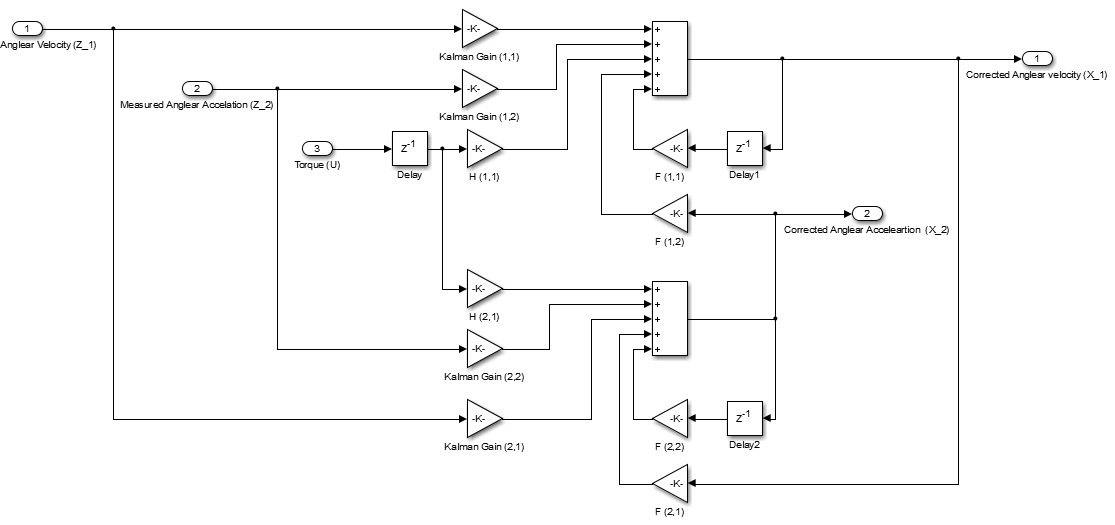
\includegraphics[scale = 0.4]{\DocRoot/images/Kalman_gordon_model}
	\caption{Simplified model of the Kalman filter}
	\label {fig: kalman used in project}
\end{figure}
